% Imported from topics/video-generation/seedance-2.5/training.md
\chapter{M13 增量训练阶段与停止条件}\label{seedance-m13}
\moduleinfo{M13}{增量路线与工程阅读；未运行教学代码}{\hyperref[src-seedance-1.0]{\texttt{seedance-1.0}}、\hyperref[src-seedance-1.5-pro]{\texttt{seedance-1.5-pro}}、\hyperref[src-wan-2.1]{\texttt{wan-2.1}}、\hyperref[src-long-context-tuning]{\texttt{long-context-tuning}}、\hyperref[src-dancegrpo]{\texttt{dancegrpo}}、\hyperref[src-rewarddance]{\texttt{rewarddance}}、\hyperref[src-diffsynth-code]{\texttt{diffsynth-code}}、\hyperref[src-longlive-code]{\texttt{longlive-code}}、\hyperref[src-ltx-code]{\texttt{ltx-code}}、\hyperref[src-dancegrpo-code]{\texttt{dancegrpo-code}}}


训练一个完整视频基础模型，与在现有模型上增加业务能力，需要完全不同的数据和预算。对于可控参考、局部编辑和多镜头任务，更容易执行的路线是保留已训练好的基座，先证明数据与损失链路正确，再逐项增加能力。

下面给出以 Wan-2.1 T2V-1.3B 为候选基座的训练流程。参数是初始试验配方，尚未经过实际训练验证；是否扩大训练，取决于每阶段的测量结果。

本流程面向较轻的视频增量试验。需要训练统一参考、编辑、结构条件和原生音视频时，采用单独的 \hyperref[seedance-m20]{联合候选训练配方}，与相应 \hyperref[seedance-m19]{完整架构} 配套；Wan 阶段的 latent、参数组和优化器状态不能直接挪用。

\section{训练阶段为什么要分开}\label{seedance-m13-ux8badux7ec3ux9636ux6bb5ux4e3aux4ec0ux4e48ux8981ux5206ux5f00}

典型生成系统先通过预训练学习宽分布，再用继续训练、高质量 SFT 和反馈优化强化能力；高分辨率精修模型也可能有自己的训练路径。

\begin{figure}
\centering
\pandocbounded{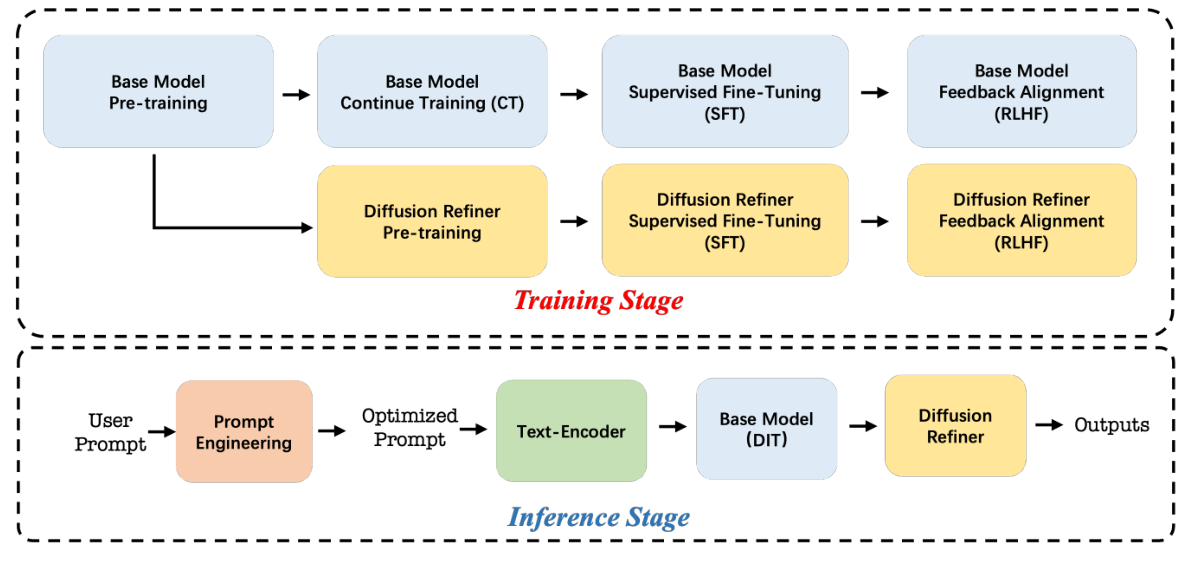
\includegraphics[keepaspectratio,alt={基础模型与精修模型的训练及推理组织 （论文示意，来源：seedance-1.0）}]{assets/seedance/figures/training-pipeline.png}}
\caption{基础模型与精修模型的训练及推理组织 （论文示意，来源：seedance-1.0）}
\end{figure}

分阶段的作用是改变数据分布、训练目标或可训练参数，同时保留上一步的能力。它不意味着必须照搬某个大模型的全部预训练规模。预算有限时，应先完成基座适配，而不是从头复刻基础训练。

\section{第一步：证明原版模型和数据链路正确}\label{seedance-m13-ux7b2cux4e00ux6b65ux8bc1ux660eux539fux7248ux6a21ux578bux548cux6570ux636eux94feux8defux6b63ux786e}

固定源码、模型、VAE、文本编码器、scheduler 和环境版本。先运行原版生成与真实视频重建，保存固定种子的输出，记录数值精度、非确定性算子、显存和时间。

选择 32 个有权使用的真实样本作调试集，另留来源隔离的验证集。起初关闭随机增强与条件 dropout，检查模型能否过拟合这些样本，并测试换文本、移除参考后输出是否相应变化。调试集的重现不能作为泛化成绩，但能快速发现目标符号、latent 缩放和条件接线错误。

必须测到有效样本/秒、有效 token/秒、step 时间、峰值显存和梯度范数，才有依据确定后续 batch、分辨率和预算。

\section{第二步：只训练图片参考支路}\label{seedance-m13-ux7b2cux4e8cux6b65ux53eaux8badux7ec3ux56feux7247ux53c2ux8003ux652fux8def}

冻结原 VAE、文本编码器和主干，训练参考特征投影、池化、角色嵌入和门控交叉注意力。先保留纯文本任务作回归，再比较少量主干 LoRA 是否带来额外收益。

{\def\LTcaptype{table} % do not increment counter
\small\setlength{\tabcolsep}{3pt}\renewcommand{\arraystretch}{1.18}
\begin{longtable}[]{@{}
  >{\raggedright\arraybackslash}p{(\linewidth - 2\tabcolsep) * \real{0.2200}}
  >{\raggedright\arraybackslash}p{(\linewidth - 2\tabcolsep) * \real{0.7800}}@{}}
\toprule\noalign{}
\begin{minipage}[b]{\linewidth}\raggedright
项目
\end{minipage} & \begin{minipage}[b]{\linewidth}\raggedright
初始候选
\end{minipage} \\
\midrule\noalign{}
\endhead
\bottomrule\noalign{}
\endlastfoot
输入桶 & 例如 \(256\times448\)、33 帧；需符合实际基座和预处理约定 \\
精度 & 硬件支持时 BF16 \\
优化器 & AdamW，学习率 \(10^{-4}\)，\(\beta=(0.9,0.999)\)，\(\epsilon=10^{-8}\) \\
权重衰减 & 0.01 \\
有效全局 batch & 8 个样本 \\
梯度裁剪 & 全局范数 1.0，同时记录裁剪前范数 \\
预热与步数 & 预热 100 步，总计 1000 步的 pilot \\
条件 dropout & 文本与参考各 0.1，独立采样 \\
验证与保存 & 每 100 步固定验证，保存可恢复状态与独立最佳点 \\
\end{longtable}
}

全局 batch 由单卡 microbatch、梯度累积和卡数共同决定：

\[
B_{\mathrm{global}}=B_{\mathrm{micro}}\times K_{\mathrm{accum}}\times N_{\mathrm{GPU}}.
\]

目标 batch 为 8、每卡 microbatch 为 1 时，累积步数需与卡数匹配，不能简单使用向下取整悄悄改变有效 batch。损失应按有效元素归一化，避免长片或大图仅因 token 更多而主导更新。

低分辨率可以降低验证成本，但形状合法不等于分布适配。身份改善、动作退化和纯文本回归都要通过固定任务集观察。随机裁剪、位置变换和更大分辨率应在基线正确后逐项加入，并同步变换 mask 与框。

\section{第三步：训练区域和区间编辑}\label{seedance-m13-ux7b2cux4e09ux6b65ux8badux7ec3ux533aux57dfux548cux533aux95f4ux7f16ux8f91}

新增源条件支路，输入源 latent、编辑与上下文 mask、修改指令和可选参考。先冻结已验证的参考支路，在受控重渲染真值上验证，再混入人工真实编辑对和弱监督数据。

起步任务可以是服装颜色、局部物体和背景替换；相机视角、全局光照和复杂遮挡另立切片。损失掩码、非目标保持损失以及最终像素合成要明确分工。latent 一致不保证像素无变化，外区直接复用也不保证边缘光照自然。

只有目标变化、外区保持和时间边界同时改善，才扩大训练；否则应先回到数据配对、mask 和任务约束，而不是立即用更复杂奖励压高总分。

\section{第四步：扩大到场景级多镜头}\label{seedance-m13-ux7b2cux56dbux6b65ux6269ux5927ux5230ux573aux666fux7ea7ux591aux955cux5934}

先做两镜头，再做四镜头，样本包含全局角色与环境、逐镜头动作、道具状态和时间顺序。按 token 预算组 batch，跨场景 packing 使用隔离 mask，避免不同故事互相读取。

异步噪声需要逐镜头噪声时间与相应调制。如果基座仅支持全局 timestep，必须增加并训练正确的逐 token 条件，而不是只替换 attention mask。

双向场景模型先作为联合生成对照，因果续写另做适配并独立保存版本。缓存先通过完整重算等价检查，再测速度。训练时逐步加入自生成历史，观察它与真实历史之间的分布差异；长程评测按时间段看漂移，不能只报告整段平均。

\section{第五步：把联合音频作为独立工程}\label{seedance-m13-ux7b2cux4e94ux6b65ux628aux8054ux5408ux97f3ux9891ux4f5cux4e3aux72ecux7acbux5de5ux7a0b}

需要先确定音频 codec 和主干，明确采样率、token rate、延迟与授权数据。先冻结视频，训练音频及跨模态门控，再根据同步和音质收益决定是否联合解冻。

缺失音轨的样本不计算音频目标，真实静音保留监督。嘴形、动作音效、语言、音色和音乐控制分别评估；不能只因为音轨时长对上，就认为联合生成已经正确。

\section{偏好优化和蒸馏放在哪一步}\label{seedance-m13-ux504fux597dux4f18ux5316ux548cux84b8ux998fux653eux5728ux54eaux4e00ux6b65}

先做高质量 SFT，再验证固定候选的奖励重排是否与人工一致。奖励可靠后才考虑 RL；低步数蒸馏再以已确定的 teacher 和任务分布展开。生成器、奖励模型、数据和 student 都需独立版本，防止边训练边换评价标准。

若奖励上涨但人工通过率下降，或者动作和构图趋于单一，应停止回滚。少步数 student 也需要与 teacher 比较身份、动作与交付可用率，不能只比较每秒出多少帧。

\section{怎样保证训练能恢复、成本能估算}\label{seedance-m13-ux600eux6837ux4fddux8bc1ux8badux7ec3ux80fdux6062ux590dux6210ux672cux80fdux4f30ux7b97}

保存模型权重之外，还要保存 optimizer、scheduler、全局步数、所有随机状态、数据采样位置和梯度累积状态。一次中断后，应对照不中断运行的下一批样本 ID 与损失，验证恢复语义。只加载权重继续跑不等于精确续训。

预算依据实测 step 时间计算：

\[
T_{\mathrm{hours}}=\frac{N_{\mathrm{steps}}t_{\mathrm{step}}}{3600},
\qquad
C_{\mathrm{GPU\,hours}}=T_{\mathrm{hours}}N_{\mathrm{GPU}}.
\]

还要另计数据制作、验证、checkpoint 和失败重跑。学习率、有效 batch、分辨率和训练参数范围改变后，吞吐可能重新变化；预算应随测量更新，而不是由模型参数量单独推断。

\section{真实工程从哪里进入}\label{seedance-m13-ux771fux5b9eux5de5ux7a0bux4eceux54eaux91ccux8fdbux5165}

LoRA 与全参训练先从 \href{https://github.com/modelscope/DiffSynth-Studio/blob/d32f72424cd22bc0ea8100cc57559149b4eac933/examples/wanvideo/model_training/train.py}{DiffSynth Wan train.py} 和 \href{https://github.com/modelscope/DiffSynth-Studio/blob/d32f72424cd22bc0ea8100cc57559149b4eac933/examples/wanvideo/model_training/lora/Wan2.1-T2V-1.3B.sh}{LoRA 配方} 阅读；流式长训练看 \href{https://github.com/NVlabs/LongLive/blob/31c70d9071cd7851d82939806dc9fac645fcabe5/LongLive1.0/pipeline/streaming_training.py}{LongLive1.0 streaming\_training}；联合音视频看 \href{https://github.com/Lightricks/LTX-2/blob/daa6b16fc7f0f1628f2c9e36a303e3312b333cc6/packages/ltx-trainer/README.md}{LTX trainer}；策略优化看 \href{https://github.com/XueZeyue/DanceGRPO/blob/15cc71d53cc2e6e18a68ee607d5fb6ba9a99e344/fastvideo/train_grpo_hunyuan.py}{DanceGRPO 视频训练}。这些是各自框架中的真实入口，环境、数据和权重按对应版本匹配，未在此执行训练。
